\section{JOGOS}
%{{{
Segundo \autocite{indieGamesLemes} jogo digital constitui-se em uma
atividade lúdica composta por uma série de ações e decisões,
limitada por regras e pelo universo do game, que resultam em uma
condição final.

Apesar de haver muita pesquisa sobre os malefícios dos games , existe
uma gama crescente de estudos apontando os benefícios dos jogos. Video
games melhoram as funções cognitivas, as capacidades criativas, e
motivam uma visão positiva diante a falha \autocite{gamebenefits}.
Também segundo \autocite{gamebenefits} postura positiva em relação a
falha correlaciona-se com melhor performance acadêmica.

A natureza dos jogos tem mudado drasticamente na última década, se
tornando cada vez mais complexos, diversos, realísticos e sociais em
sua natureza \autocite{gamebenefits}. Apesar de a mídia ter criado
uma perspectiva negativa sobre jogos, especialmente os violentos, a
realidade é mais complexa do que se demonstra.

Jogadores de jogos violentos, que encorajem jogabilidade cooperativa,
são mais prováveis de exibir comportamento altruísta fora do
contexto dos jogos, do que jogadores de jogos não violentos
\autocite{gamebenefits}.

Além do aspecto social, jogos tem potencial para melhorar habilidades
intelectuais dos jogadores. Jogadores de jogos de tiro demonstram maior
alocação de atenção, maior resolução espacial no processamento
visual e melhor habilidades de rotação \autocite{gamebenefits}. Estes
aspectos positivos muitas vezes não recebem méritos suficientes.
Habilidades espaciais derivadas de jogar jogos de tiro comercialmente
disponíveis são comparáveis aos efeitos de um curso universitário
que busca melhorar as mesmas habilidades \autocite{gamebenefits}. Estas
habilidades são centrais para muitas áreas de interesse humano.
Segundo \autocite{gamebenefits} habilidades espaciais está diretamente
relacionado com o sucesso em ciência, tecnologia, engenharia e
matemática.

\subsection{Jogos Web}

Jogos da WEB podem se beneficiar da estrutura social da internet.

Não há muito que os títulos de jogos da web residiam em jogos como
\textit{Traviam}, desprovidos de animações. Compostos basicamente por
formulários, imagens e textos. Não obstante, publicar jogos baseados
em texto é uma atividade cada vez mais rara, podendo-se concluir que
interface gráfica se tornou uma funcionalidade mandatória
\autocite{browserGamesTechnologyAndFuture}.

\cite{browserGamesTechnologyAndFuture} afirma que:
\begin{quote}
Estudos sugerem que flexibilidade, em essência facilidade de entrada
e saída, é uma das duas razões principais da utilização de jogos
de navegadores. A outra razão primária é o fator social envolvido no
jogo.
\end{quote}

%Mencionar algum jogo (como WOW) e como ele faz para prender a atenção dos usuários. Candy Crush saga

\subsection{GÊNEROS}

Uma classificação de jogos em gêneros é uma tarefa complexa. Segundo \autocite{gamebenefits}:

Segundo \cite[pp. 60]{gamebenefits}:
\begin{quote}
Pela diversidade em itens e gêneros e a vasta quantidade de dimensões
que os vídeo games se encontram, uma taxonomia dos jogos contemporâneos
é extremamente difícil de desenvolver (muitos já tentaram) .
\end{quote}

Não obstante alguns padrões são discerníveis quanto aos jogos da
web.

Os primeiros jogos eram limitados a tecnologias presentes, um gênero de
que se desenvolveu bem foram os jogos de estratégia como o Travian.

Com as novas possibilidades do tecnológicas novas possibilidades e
gêneros de jogos podem ser explorados na web.

\subsection{MECÂNICA}

A mecânica é composta pelas regras do jogo. Quais as ações
disponíveis aos usuários, é fortemente influenciada pela categoria do
jogo em questão.

\section{JOGOS MULTIPLATAFORMA}

Jogos em plataformas móveis trazem um novo conjunto de desafios para
produtores de jogos. Um destes desafios é fornecer feedback suficiente
para o jogador pois o dispositivo é limitado em proporções, som, tela
etc.

A interface tem que ser o mais intuitiva o possível. No caso de
dispositivos móveis, quanto menos gestos necessários melhor. Tornar
previsível causa e efeito é uma boa característica para os jogos.
Os desenvolvedores tem que evitar fazer o jogo para eles mesmos. E
pela falta de crítica os designs tendem a ser ruins. Afinal o que os
jogadores querem? LEMES (2009, pg XX) aponta alguns fatores procurados
pelos usuários de jogos: Desafio, socializar, experiência solitária,
respeito e fantasia.

Designers de jogos tem as seguintes possibilidades arquiteturais
quando em face de desenvolver um novo jogo: Criar um jogo web,
um jogo híbrido, ou nativo. As opções serão descritas abaixo.

\subsection{JOGOS WEB}

Um jogo web é um jogo que utiliza o HTML e ferramentas correlacionadas
para sua construção. Este tipo de jogo é o que será abordado neste
trabalho.

Entre seus pontos positivos pode-se listar:

\begin{itemize}
\item Necessitam de uma única base de código e pode rodar em todas as
plataformas;
\item Contém a mais vasta gama de desenvolvedores e muitos
interessados em aprendê-la;
\item Seus custos são inferiores, aos do desenvolvimento nativo devido a
inexistência de duplicação da base de código;
\item  Não requerem instalação ou atualizações manuais
\item  Sua distribuição é superior ao estilo convencional de aplicações desktop \autocite{browserGamesTechnologyAndFuture}
\end{itemize}

Os pontos negativos dessa abordagem são o principal foco deste trabalho.

Mas a um nível macroscópico podemos citar:
\begin{itemize}
\item Programas que rodam na web são geralmente lentos se comparados aos
nativos;
\item Por falta de especificação ou incompletude de implementação.
\item Nem todos os recursos disponíveis através das SDK's nativas estão presentes através do HTML5.
\end{itemize}

Além dos jogos web, há a possibilidade de criar jogos híbridos e nativos.

\subsection{JOGOS HÍBRIDOS}

Jogos híbridos são jogos geralmente desenvolvidos com tecnologias da
web que rodam nativamente.

\subsection{DESENVOLVIMENTO DE JOGOS NATIVOS}

Pontos fortes:
\begin{itemize}
\item Habilita a melhor experiência de usuário pois permite utilizar ao
máximo os recursos e funcionalidades dos dispositivos.
\end{itemize}

Pontos fracos:
\begin{itemize}
\item Porém, devido a cada plataforma conter seu próprio sistema operacional,
com seus próprios *SDK's* totalmente incompatíveis, os desenvolvedores são
forçados a desenvolver uma versão do jogo para cada plataforma alvo.
\item Requer mais pessoas, e maior custo com possivelmente parte do
mercado não atendido de qualquer forma.
\end{itemize}

%}}}
\section{WEB}
%{{{

\subsection{OPEN WEB}
A OWP (\textit{Open Web Platform}) é uma coleção de tecnologias
livres, amplamente utilizadas e padronizadas. Quando uma tecnologia se
torna amplamente popular, através da adoção de grandes empresas e
desenvolvedores, ela se torna candidata a adoção pela OWP.

Mais do que um conjunto de tecnologias Open Web, é um conjunto
de filosofias e ideias as quais a web se fundamenta. Transparência,
imparcialidade nos processos de criação e padronização de novas
tecnologias. Retro compatibilidade com as especificações anteriores.
Consenso entre o mercado e o meio acadêmico, nunca um distanciando-se
muito do outro, entre outas características.

A W3C é a empresa responsável por grande parte das especificações
da web como: HTML (em conjunto com a WHATWG), CSS, entre outros.

O processo da W3C consiste na elaboração de rascunhos de
(\textit{working drafts}) que passam por vários passos de revisão até
se tornarem recomendações. As recomendações podem ser implementadas
com segurança de que a especiação não mudará substancialmente.
Apesar do processo ser rigoroso, está longe de perfeito. A
especificação final do HTML4 contava com quatro erros publicados
via errata \autocite{HTML5}. Uma lista completa das especificações
mantidas pela W3C pode ser encontrada em: http://www.w3.org/TR/.

Outras empresas estão envolvidas nas especificações da web, como a
ECMA, responsável pelo JavaScript; Kronos, responsável pelo WebGL,
etc.

A tecnologia chave que inaugurou e alavancou este processo é o HTML.
%}}}
\section{HTML}
%{{{

HTML (\textit{Hyper Text Markup Language}) é uma linguagem de
marcação que define a estrutura semântica do conteúdo das páginas
da web. Criada por Tim Berners Lee em 1989 no CERN. HTML é a tecnologia
base para a criação de páginas web e aplicativos online. A parte
denominada: "\textit{Hyper Text}", refere-se a links que conectam
páginas HTML umas as outras, fazendo a Web como conhecemos hoje
\autocite{mdn2015}.

A última versão do HTML é o HTML5, iniciado pela WHATWG e
posteriormente desenvolvido em conjunto com a W3C. Seu rascunho foi
proposto em 2008 e ratificado em 2014. Após 2011, a última chamada
de revisão do HTML5, a WHATWG decidiu renomear o HTML5 para HTML
\autocite{htmlIsTheNewHtml5}. Não obstante, o termo HTML5 permanece em
utilização pela W3C.

Além da nomenclatura, exitem pequenas diferenças nas especificações
da W3C e WHATWG. A W3C vê a especificação do HTML5 como algo fechado,
inclusive já iniciou o desenvolvimento do HTML 5.1. Já a WHATWG vê o
HTML5 como uma especificação viva. A postura da W3C tende a criar uma
especificação estável, já a da W3C reflete mais a realidade dos
navegadores, que nunca implementam uma versão completamente. A Mozilla
utiliza a especificação da WHATWG no desenvolvimento do Firefox e
recomenda a da W3C para sistemas que requeiram maior estabilidade. Neste
trabalho optamos pela nomenclatura da WHATWG, utilizamos o termo HTML em
detrimento a HTML5, sempre que semanticamente viável.

HTML foi especificado baseando-se no padrão SGML (\textit{Standard Generalized
Markup Language}).

Alguns benefícios do SGML são:
\begin{itemize}
    \item Documentos declaram estrutura, diferentemente de aparência
, possibilitando otimizações nos ambientes de uso (tamanho de tela,
etc);
    \item São portáveis devido a definição de tipo de documento
(\textit{document type declaration});
\end{itemize}

Apesar de o SGML especificar a não definição de aparência, os criadores de
navegadores constantemente introduziam elementos de apresentação como o
piscar, itálico, e negrito, que eventualmente acabavam por serem inclusos
na especificação. Foi somente nas últimas versões que elementos de
apresentação voltaram a ser proibidos reforçando as propostas chave
do HTML como uma linguagem de conteúdo semântico, incentivando a
utilização de outras tecnologias como o CSS para responder as demandas de
apresentação.

Além do HTML, existe o XHTML, que é uma iniciativa de utilização de
XML nas páginas da web. O XML é um padrão mais rigoroso que SGML e
resulta em páginas sem problemas de sintaxe e tipografia. 
Alguns estimam que 99\% das paginas HTML de hoje
contenham ao menos um erro de estrutura \autocite{diveIntohtml}.
Uma das maiores vantagem do XML é que sistemas sem erros de sintaxe
que podem ser facilmente interpretadas por outras tecnologias como
sistemas de indexação, buscadores, etc.

Para transformar o HTML em algo visível os navegadores utilizam motores
de renderização. O primeiro passo efetuado por esses sistemas é
decodificar o documento HTML para sua representação em memória. Este
processo dá-se através da análise (\textit{parsing}) e posterior
tokenização, que é a separação do HTML em palavras chave que o
interpretador pode utilizar. Diferentemente do XHTML, HTML não pode
ser decodificado através de tokenização tradicional. Deve-se ao HTML
ser amigável ao programador, aceitando erros de sintaxe, dependente
de contexto, buscando entregar a melhor aproximação possível. 
Segundo \cite{howBrowsersWork} essa é a maior razão do HTML ser tão popular - 
ele perdoa os erros e torna a vida dos autores da WEB mais fácil. Esta
característica deu origem a uma especificação para renderizar HTML
(\textit{HTML parser}).

Antes do HTML5 várias versões foram propostas, algumas radicais
em seus preceitos. O XHTML 2.0, por exemplo, quebrava com toda
a compatibilidade das versões anteriores e acabou por sendo descontinuado.
Outrossim, a maioria das versões HTML de grande sucesso foram versões de
retrospectiva (\textit{retro-specs}). Versões que não tentavam
idealizar a linguagem, buscando alinhar-se com os requerimentos do
mercado \autocite{diveIntohtml}. Não obstante, a ideia que a melhor forma
de ajustar o HTML é substituindo ele por outra coisa ainda aparece de tempos
em tempos \autocite{diveIntohtml}.

Uma página HTML consiste em elementos que podem ter seu comportamento
alterado através de atributos. Um elemento é o abrir fechar de
uma tag e todo o conteúdo que dentro dele reside \autocite[pp.
10--11]{htmlAndCssDucket}. Por exemplo, na figura \ref{fig:htmlSample} o elemento
meta (<meta>) tem um atributo \textit{charset}, que especifica o formato de 
codificação do documento.

\begin{figure}
\centering
\begin{verbatim}
<}!DOCTYPE HTML>
<html lang="en-US">
<head>
	<meta charset="UTF-8">
	<title></title>
</head>
<body>
    <video>
        <span>Seu navegador não suporta vídeo</span>
    </video>
</body>
</html>
\end{verbatim}
\caption{Exemplo] de documento HTML}
\label{fig:htmlSample}
\end{figure}


Na sua versão inicial, o HTML contava com 18 elementos; atualmente
existem aproximadamente cem \autocite{diveIntohtml}. Não obstante, foi
no HTML5 que a maior parte dos elementos que viabilizam a construção
de jogos foram adicionados.

Uma das características do HTML que o torna tão popular é seu
interesse em manter manter a retrocompatibilidade. Interpretadores
HTML atingem isso ignorando os elementos que não conhecem, tratando
seu vocabulário exclusivamente. Esse mecanismo permite que os
desenvolvedores incluam marcação de reserva dentro dos elementos
que podem não ser suportados. O elemento \textit{span} na figura
\ref{fig:htmlSample} só aparecerá para o usuário caso seu navegador
não suporta a tag vídeo.

Além da convencional linguagem de marcação, HTML é muitas vezes
interpretado como um conceito guarda chuva para designar as tecnologias
da web. Segundo \autocite{diveIntohtml} algumas dessas tecnologias (como geolocalização) estão em especificações separadas mas são tratadas como HTML5 também. Outras
tecnologias foram removidas do HTML5 estritamente falando, mas são tratados
como HTML5 (como a API de armazenamento de dados).

\begin{figure}
    \centering
    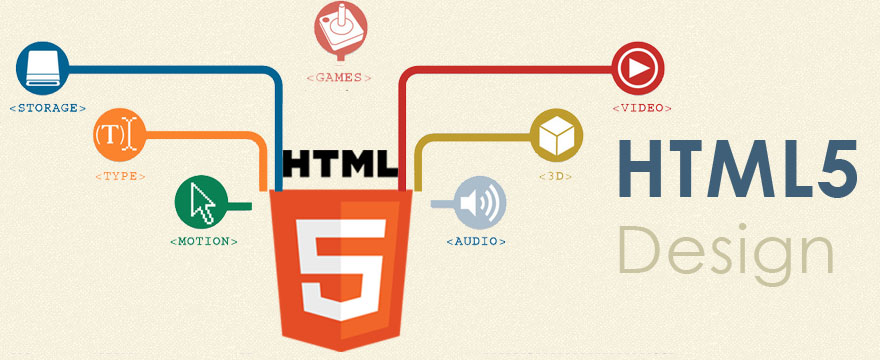
\includegraphics[width=0.8\textwidth,natwidth=610,natheight=642]{html5.jpg}
    \caption{Suíte HTML}
\end{figure}

Uma tecnologia fortemente entrelaçada com o HTML é o DOM. Tendo uma relação próxima de um para um com a marcaçaõ \autocite{howBrowsersWork}. DOM permite a interação entre documentos HTML e as demais tecnologias da WEB de uma forma fácil e padronizada.

\subsection{DOM}
%{{{

O modelo de documento de objetos (\textit{Document Object Model}) é
a representação em memória de uma árvore de elementos HTML. Esta
representação é definida por um conjunto de padrões que torna
interoperável a manipulação de elementos através de JavaScript.

A primeira versão do DOM, DOM nível zero, foi parcialmente
especificada no HTML 4 e permitia manipulação parcial dos elementos.
Foi somente com a especificação do JavaScript em 1998 que o DOM nível
1 foi especificado, permitindo a manipulação de qualquer elemento. DOM
nível 2 e 3 seguiram com melhorias nas consultas aos elementos e CSS.

A API de seletores do DOM permite alto nível de precisão e performance
para buscar elementos

\begin{figure}
\centering
\begin{verbatim}
    var elementos = document.querySelector( ".main, #sceen"  );
    var elementosB = document.querySelectorAll( "a.minhaClasse, p"  );
\end{verbatim}
\caption{Exemplo de utilização de seletores do DOM em JavaScript}
\label{fig:selectorsSample}
\end{figure}

A figura \ref{fig:selectorsSample} demonstra a utilização dos seletores do DOM em um documento
JavaScript. O método \textit{querySelector} seleciona o primeiro elemento em conformidade
com o padrão especificado. Já o método \textit{querySelectorAll} seleciona todos os elementos
que estão em acordo com o padrão especificado.

%}}}
%}}}
\section{CSS}
%{{{
CSS (\textit{Cascading Style Sheets}) é uma linguagem de folhas de
estilo criada por Håkon Wium Lie em 1994 com intuito de definir a
apresentação de páginas HTML. CSS, juntamente com JavaScript e HTML,
compõem as tecnologias centrais no desenvolvimento WEB tornando-se
parte da OWP; sua especificação é atualmente mantida pela W3C.

O termo \textit{Cascading} refere-se ao fato de regras serem herdadas
pelos filhos de um elemento, eliminando grande parcela de duplicação
antes necessária para estilizar uma página. A diferenciação entre
apresentação e estrutura, sendo neste caso o CSS responsável pela
apresentação, é um dos pontos chave do SGML, motivo que tornou a
utilização do CSS tão conveniente para o desenvolvimento WEB.

Antes do CSS era impossível ter estilos diferenciados para diferentes
tipos de dispositivos, limitando a aplicabilidade dos documentos.
Com CSS também tornou-se possível que o usuário declare suas próprias
folhas de estilo, um recurso importante para acessibilidade.

Segundo \cite[pp. 23--24]{CascadingStyleSheets}:

\begin{quote}
CSS possibilita a ligação tardia (\textit{late biding}) com
páginas HTML. Essa característica é atrativa para os publicadores
por dois motivos. Primeiramente pois permite o mesmo estilo em várias
publicações, segundo pois os publicadores podem focar-se no conteúdo
ao invés de se preocuparem-se com detalhes de apresentação.
\end{quote}

CSS é formado por um conjunto de regras, dentro de uma tag HTML
denominada \textit{style}, que são agrupadas por seletores em blocos
de declaração. Os elementos selecionados são denominados o assunto
do seletor \autocite{cssSelectors}. Seletores tem o intuito de definir
quais partes do documento HTML serão afetadas por determinado bloco de
declaração.

A figura \ref{fig:CSSSample} exemplifica este processo. O seletor em
questão é o elemento \textit{<p>}, simbolizando todos os parágrafos. O bloco de
declaração é o que está dentro das chaves, aplicando alinhamento e
cores aos parágrafos.

\begin{figure}
\centering
\begin{verbatim}
<style>
p {
    text-align: center;
    color: red;
}
</style>
\end{verbatim}
\caption{Exemplo de Folha de Estilo}
\label{fig:CSSSample}
\end{figure}

CSS é dividido em módulos, que representam conjuntos de
funcionalidades, contendo aproximadamente 50 deles. Cada módulo evolui
separadamente, esta abordagem é preferida pois permite uma maior
entrega de novas funcionalidades, pois novos recursos não dependem da
aceitação de outros para serem disponibilizados.

Além do módulos, CSS também é organizado por perfis e níveis.

Os perfis do CSS organizam a especificação por dispositivo de utilização.
Existem perfis para dispositivos móveis, televisores, impressoras, etc.
Existem conjuntos de regras que se aplicam somente a uma classe de dispositivos,
ou que sofrem alterações nas regras conforme as regras.

Já os níveis organizam o CSS por camadas de abstração. Os níveis
inferiores representam as funcionalidades vitais do CSS, os níveis
superiores dependem dos inferiores para construir as funcionalidades
elaboradas.

A primeira especificação do CSS, CSS1 (ou nível 1) foi lançada em
1996. Em 1997 foi lançado o CSS2 com o intuito de ampliar a completude
do CSS1. Em 1998 iniciou-se o desenvolvimento do CSS3 que ainda continua
em 2015. Além do nível 3 existem módulos de nível 4 no CSS, não
obstante o termo CSS3 ainda é o mais utilizado.

Apesar da clara evolução das versões do CSS, esse processo nem
sempre é linear. Em 2005 o grupo de trabalho do CSS decidiu aumentar a
restrição de suas especificações rebaixando o CSS 2.1, Seletores do
CSS3 e Texto do CSS3 de recomendações para rascunhos.

\begin{figure}
    \centering
    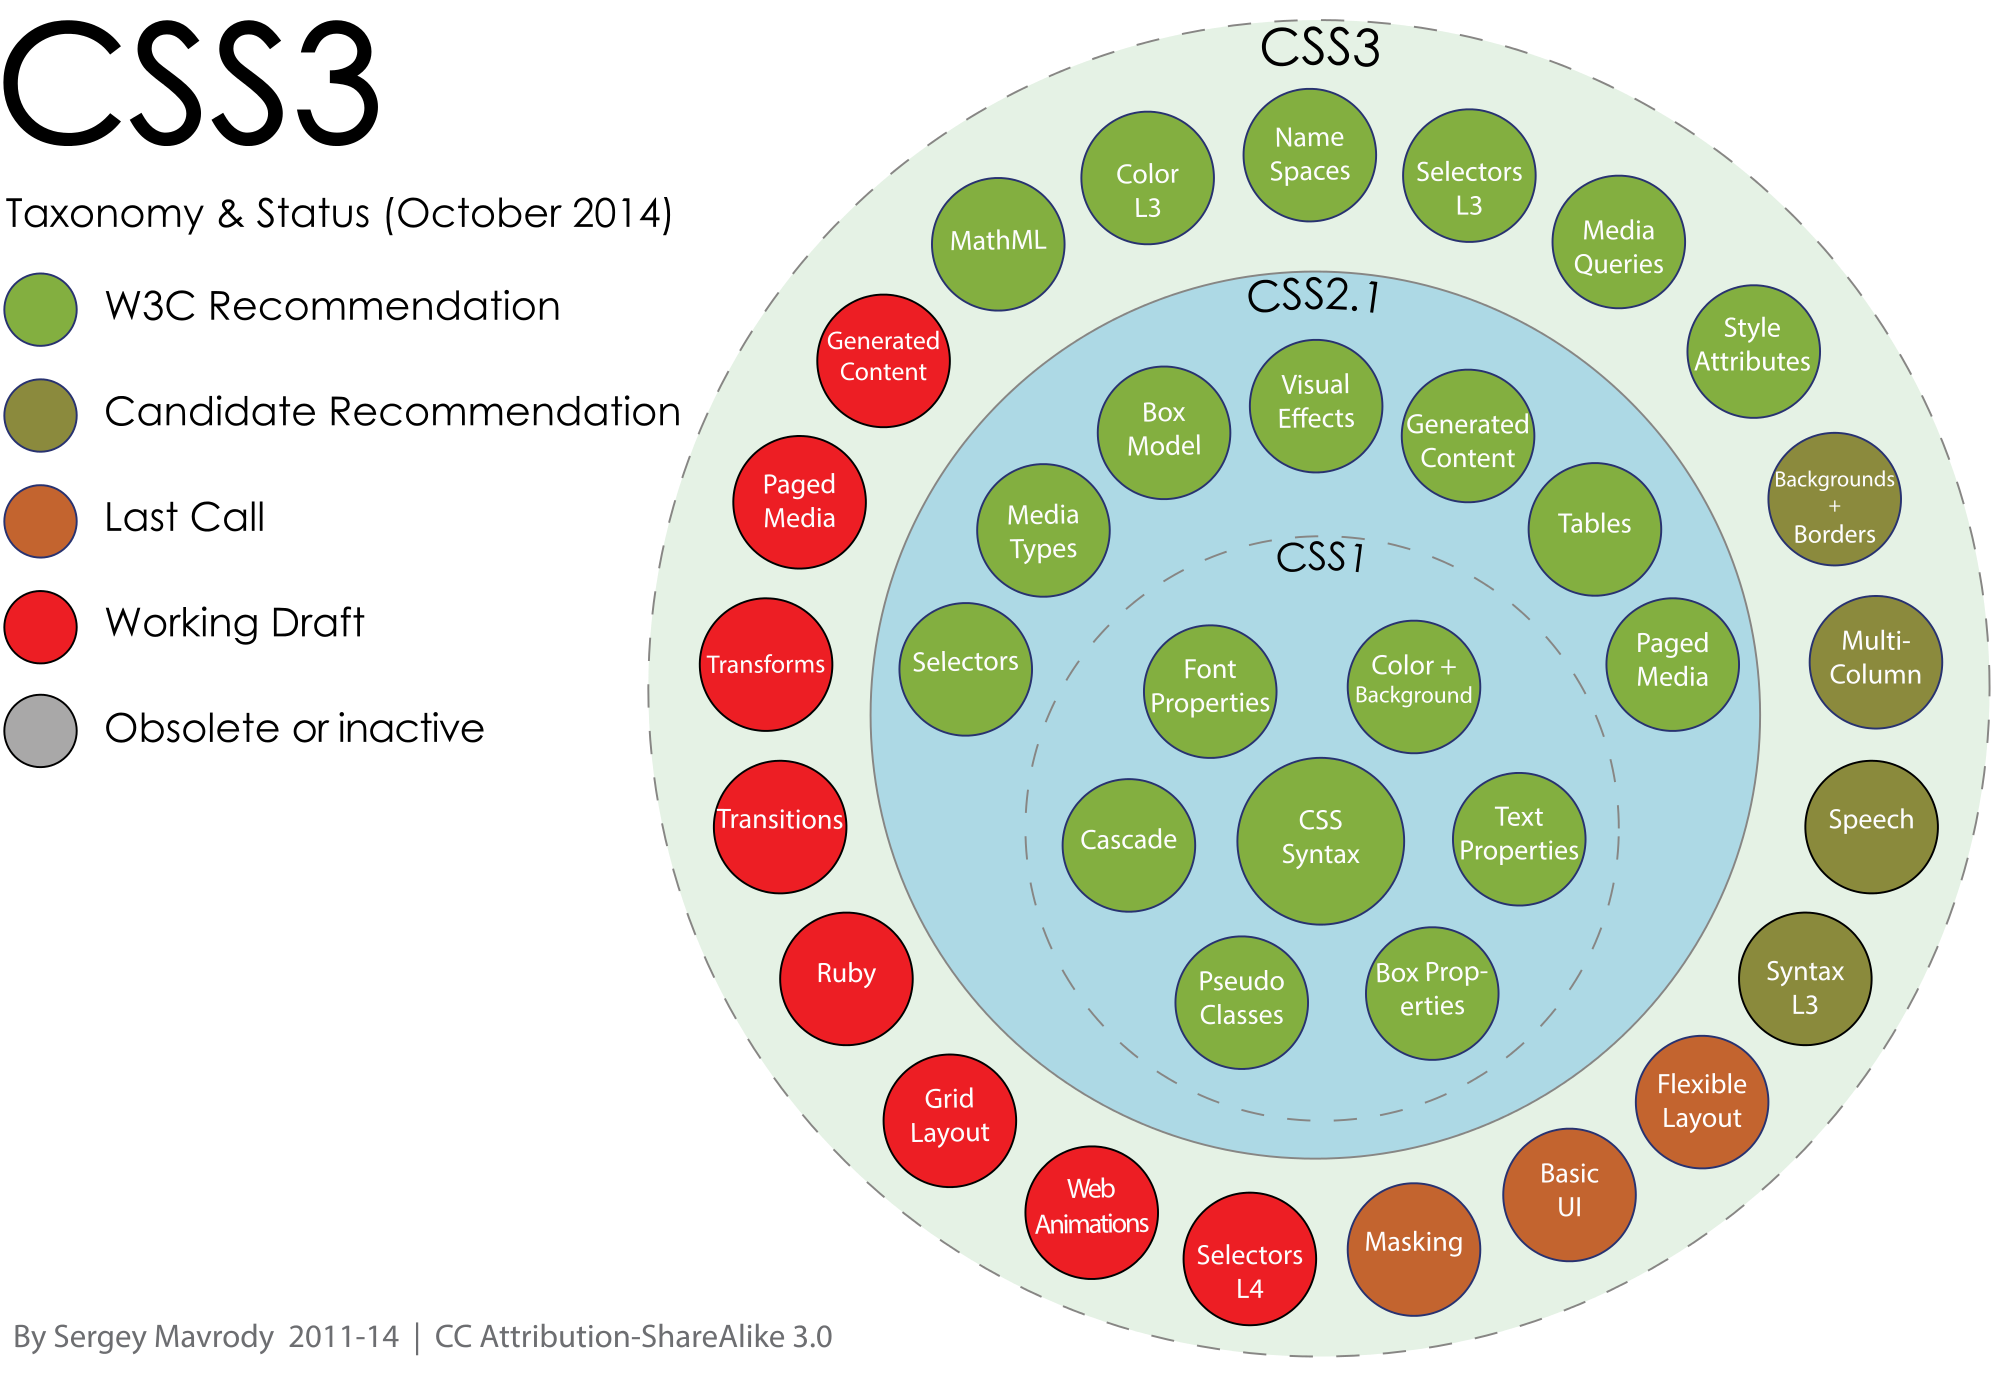
\includegraphics[width=0.8\textwidth,natwidth=610,natheight=642]{cssModules.png}
    \caption{Os módulos do CSS}
    \source{https://commons.wikimedia.org/wiki/File:CSS3\_taxonomy\_and\_status-v2.png}
\end{figure}

O CSS3, introduziu várias funcionalidades relevantes para jogos, como
\textit{media-queries}, transições, transformações 3D, entre outros.

\subsection{Media Queries}

Media Queries permitem aplicar regras a dispositivos específicos,
dependendo de suas capacidades, como resolução, orientação, tamanho
de tela, entre outros.

A especificação prevê a possibilidade de aplicar seletores entro
de arquivos CSS, ou aplicar arquivos inteiros dependentemente das
configuração do aparelho em questão.

\begin{figure}
\centering
\begin{verbatim}
@media only screen and (min-width: 1024px) {
    background-color: green;
}
\end{verbatim}
\caption{Exemplo de Media Query}
\label{fig:MediaQuery}
\end{figure}

A figura \ref{fig:MediaQuery} demostra a aplicação de uma regra via
seletor Media Query, aplicando o a cor de fundo para dispositivos com no
minimo 1024 px de resolução.

CSS nível 4 permite a utilização de media queries (\textit{Custom
Media Queries}) criados pelo usuário, com regras e definições
customizadas. A figura \ref{fig:MediaQueryCustom} demostra as novas
possibilidades de definição de media queries tanto em CSS como em
JavaScript.

\begin{figure}
\centering
\begin{verbatim}
@custom-media --narrow-window (max-width: 30em);

<script>
CSS.customMedia.set('--foo', 5);
</script>

\end{verbatim}
\caption{Exemplo de media queries customizados}
\label{fig:MediaQueryCustom}
\source{https://developer.mozilla.org/en-US/docs/Web/CSS/MediaQueries}
\end{figure}

%falar de tamanhos absolutos vs relativo
%Unidades vw e vh para tamanho do viewport

\subsection{Transições}

É uma forma de adicionar animações em uma página web.
Estas animações são compostas por um estado inicial e um
final. A especificação de transições permite grande controle
sobre a transição. Habilitando o desenvolvedor a controlar
o tempo de execução os estados intermediários de uma transição.

Atualmente um conjunto finito de propriedades podem ser animadas
com transições, e essas lista tende a mudar com o tempo, cabe ao
desenvolvedor assegurar-se que determinada propriedade está disponível
\autocite{mdnTransitions}.

Transições são interessantes em jogos, especialmente pois muitos
navegadores suportam aceleração de GPU (Unidade de processamento
gráfico) para estas operações. Isso garante grandes benefícios de
performance sobre implementações diretamente em JavaScript.

\begin{figure}
\centering
\begin{verbatim}
<style>
.test:hover
{
        -webkit-transform: scale(1.2);
        -ms-transform: scale(1.2);
        transform: scale(1.2);
}
</style>
\end{verbatim}
\caption{Exemplo de transição}
\label{fig:CSSTransition}
\end{figure}

A transição demonstrada na figura \ref{fig:CSSTransition} escala o
tamanho do elemento com a classe (\textit{test}) para vinte porcento a
mais do seu tamanho original. Perceba também os comandos repetidos com
o prefixo ms e WebKit. Esse tipo de abordagem é comum para tecnologias
que não passam de rascunhos na especificação.

Navegadores tentam otimizar a experiência de navegação definindo
um conjunto de regras e configurações razoáveis para a maioria dos
casos. Não obstante, nem sempre estes valores padrões são as melhores
opções no contexto de jogos. Abaixo segue uma lista de configurações
interessantes para se fazer com CSS no contexto de desenvolvimento de
jogos.
%\subsection{Transformações 3D}

\subsection{CSS 4}

Apesar de o termo CSS 4 ser bastante utilizado, o grupo de trabalho do CSS
não considera mais a existência de versões, como foi até o CSS3.
Não obstante existem recursos cuja especificação está avançada e não estavam presentes
no CSS 3 quando este foi lançado, dentre estas funcionalidades inclui-se:

\begin{itemize}
\item Suporte a variáveis no CSS
\item Media queries customizadas
\item Funções de cores como: color(), hwb() e gray()
\item Suporte a filtros
\end{itemize}

Recursos recentes do CSS muitas vezes não estão presentes nos
navegadores, não obstante muitos deles são interessantes no contexto
de desenvolvimento de jogos, como o suporte a variáveis.

O projeto cssnext http://cssnext.io/ é uma iniciativa para permitir a
utilização dos recentes recursos do CSS mesmo sem os mesmos estarem
implementados nos navegadores. O projeto funciona compilando o código
não suportado em algo compatível com versões para as versões
implementadas pelos navegadores.

Além da apresentação, recurso vital para jogos, e aplicativos web em
geral, é a iteratividade. Com as tecnologias da WEB esta iteratividade
é atingida através do JavaScript.
%}}}
\section{JAVASCRIPT}
%{{{

EMACScript, melhor conhecida como JavaScript, criada por Brendan Eich em
1992, é a linguagem de script da Web. Devido a tremenda popularidade
entre comunidade de desenvolvedores a linguagem foi abraçada pela W3C e
atualmente é um dos componentes da Open Web.

As definições da linguagem são descritas na especificação ECMA-262.
Esta possibilitou o desenvolvimento de outras implementações além da
original (SpiderMonkey) como o Rhino, V8 e TraceMonkey; bem como
outras linguagens similares como JScript da Microsoft e o ActionScript
da Adobe.

Segundo a \cite{ecmaSpecificaton}:
\begin{quote}
Uma linguagem de script é uma linguagem de programação que é
usada para manipular e automatizar os recursos presentes em um dado
sistema. Nesses sistemas funcionalidades já estão disponíveis
através de uma interface de usuário, uma linguagem de script é
um mecanismo para expor essas funcionalidades para um programa
protocolado.
\end{quote}

No caso de JavaScript na web, os recursos manipuláveis são o conteúdo
da página, elementos HTML, elementos de apresentação,
a própria janela do navegador e variados outros recursos que tem
suporte adicionado por novas especificações.

A intenção original era utilizar o JavaScript para dar suporte aos já
bem estabelecidos recursos do HTML, como para validação, alteração
de estado de elementos, etc. Em outras palavras, a utilização do
JavaScript era opcional e as páginas da web deveriam continuar
operantes sem a presença da linguagem.

Não obstante, com a construção de projetos Web cada vez mais complexos, as
responsabilidades delegadas ao JavaScript aumentaram a ponto que a
grande maioria dos sistemas web não funcionarem sem ele.
JavaScript não evoluiu ao passo da demanda e muitas vezes carece de
definições expressivas, completude teórica, e outras características
de linguagens de programação mais bem estabelecidas, como o C++ ou
Java \autocite{crossPlatformMobileGame}.

A última do JavaScript, o JavaScript 6, é um esforço nessa direção.
JavaScript 6 ou EMACScript Harmonia, contempla vários conceitos de
orientação a objetos como classes, interfaces, herança, tipos, etc.
Não obstante o suporte ao JavaScript 6 é apenas parcial em todos
os navegadores. O site http://kangax.github.io/compat-table/es6/
apresenta um comparativo de suporte das funcionalidades do JavaScript.

Segundo \cite{ecmaSupport} o suporte no início de 2015 era o seguinte:

\begin{itemize}
    \item Chrome: 30\%
    \item Firefox: 57\%
    \item Internet Explorer : 15\%
    \item Opera: 30\%
    \item Safari: 19\%
\end{itemize}

Estes esforços de padronização muitas vezes não são rápidos
o suficiente para produtores de software web, demora-se muito até
obter-se um consenso sobre quais as funcionalidades desejadas em
determinada versão e seus detalhes de implementação. Além da
espera por especificações, uma vez definidas, é necessário que os
navegadores especificado.

O projeto babel https://github.com/babel/babel é um compilador de
JavaScript 6 para JavaScript 5. Permitindo que, mesmo sem suporte, os
desenvolvedores possam usufruir dos benefícios da utilização do
JavaScript 6 durante o tempo de desenvolvimento, gerando código em
JavaScript 5 para rodar nos navegadores.

Alternativamente, existe uma vasta gama de conversores de código -
(\textit{transpilers}) - para JavaScript; possibilitando programar
em outras linguagens posteriormente gerando código JavaScript.
Entretanto, essa alternativa tem seus pontos fracos, necessita-se
de mais tempo de depuração, visto que o JavaScript gerado não é
conhecido pelo desenvolvedor, e provavelmente o código gerado não
será tão otimizado, nem utilizará os recursos mais recentes do
JavaScript.

Mesmo com suas fraquezas amplamente conhecidas, JavaScript está
presente em praticamente todo navegador atual. Sendo uma espécie de
denominador comum entre as plataformas. Essa onipresença torna-o
integrante vital no processo de desenvolvimento de jogos multiplataforma
em HTML5. Vários títulos renomeados já foram produzidos que fazem
extensivo uso de JavaScript, são exemplos: Candy Crush Saga, Angry
Birds, Dune II, etc.

Jogos Web são geralmente escritos na arquitetura cliente servidor,
JavaScript pode rodar em ambos estes contextos, para tanto, sua
especificação não define recursos de plataforma. Distribuidores do
JavaScript complementam a o JavaScript com recursos específicos para
suas plataformas alvo. Por exemplo, para servidores, define-se objetos como:
console, arquivos e dispositivos; no contexto de cliente,
são definidos objetos como: janelas, quadros, DOM, etc.

Para o navegador o código JavaScript geralmente é disposto no elemento
script dentro de arquivos HTML. Quando os navegadores encontram esse
elemento eles fazem a requisição para o servidor e injetam o código
retornado no documento, e a não ser que especificado de outra forma,
iniciam sua execução.

\subsection{JAVASCRIPT 7}

Antes da finalização da especificação 6, algumas funcionalidades
do JavaScript 7 já haviam sido propostas. Na página
https://github.com/tc39/ecma262 pode-se conferir os itens propostos e
seu estágio de evolução.

Alguns dos recursos esperados para o JavaScript 7 são: guards, contratos
e concorrência no laço de eventos \autocite{ecma7}.

A figura \ref{fig:ecma7} é a tabela de funcionalidades sugeridas e seu
estágio no caminho da especificação.

\begin{figure}
    \centering
    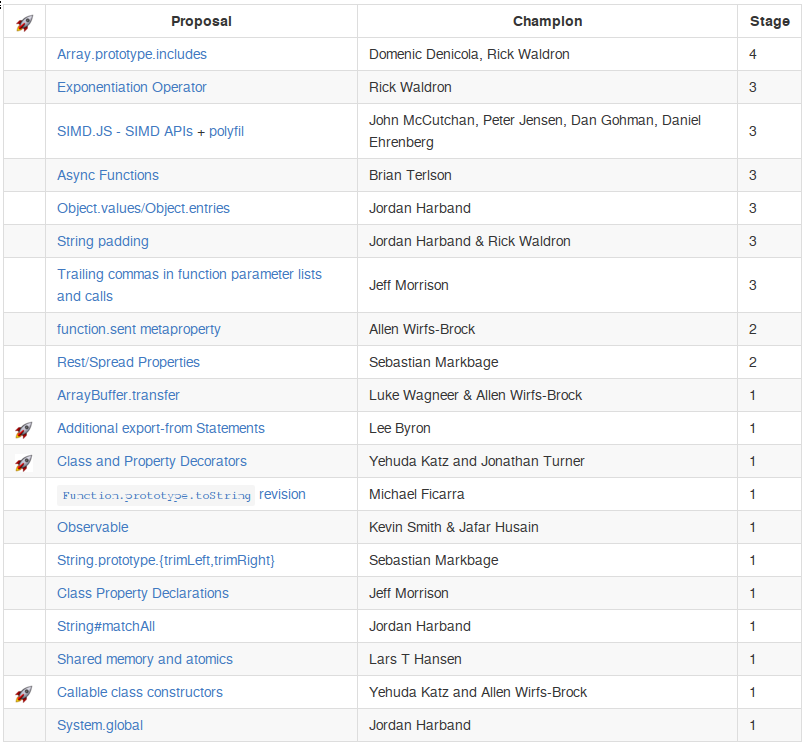
\includegraphics[width=0.8\textwidth,natwidth=610,natheight=642]{ecma7.png}
	\caption{Propostas do ECMA 7}
	\source{https://github.com/tc39/ecma262}
    \label{fig:ecma7}
\end{figure}

\subsection{ASM.JS}% o correto é asm.js

Asm.js é um subconjunto da sintaxe do JavaScript a qual permite
grandes benefícios de performance quando em comparação com
JavaScript normal. Entretanto, não é trivial escrever código em
asm.js e geralmente a criação de código asm.js é feita através
da conversão de outras linhagens como C. O projeto Emscripten
https://github.com/kripken/emscripten pode ser utilizado para gerar
código em asm.js é utilizado pelo motor de jogos Unity 3D e Unreal.

No contexto dos jogos performance é um fator de extrema importância
asm.js se destaca por utilizar recursos que permitam otimizações
antes do tempo (\textit{ahead of time optimizations}). Grade parcela
da performance adicional, em relação ao JavaScript, é devido a
consistência de tipo e a não existência de um coletor de lixo
(\textit{garbage collector}) - a memória é gerenciada manualmente
através de um grande vetor. Esse modelo simples desprovido de
comportamento dinâmico, sem alocação e desalocação de memória,
apenas um bem definido conjunto de operações de inteiros e flutuantes
possibilita grade performance e abre espaço para otimizações.

O desenvolvimento do asm.js iniciou-se no final de 2013 não obstante a
maioria dos navegadores não implementam ou implementam parcialmente o
rascunho. O motor JavaScript da Mozilla, SpiderMonkey, é a exceção,
implementando a grande maioria dos recursos do asm.js.

\subsection{WEB Assembly}

Web Assembly é uma tecnologia recentemente proposta que pretende se tornar o formato de máquina da Web.
Irá permitir que outras linguagens além do JavaScript gerem código que rode nativamente nos navegadores com grande 
ganhos de performance e flexibilidade, visto que será possível utilizar qualquer linguagem para gerar código especificado pelo Web Assembly.

WebAssembly (short: wasm) is a new binary format for the WEB, created by Google, Microsoft, Mozilla and others. It will be used for performance critical code and to compile languages other than JavaScript (especially C/C++) to the WEB platform. It can be seen as a next step for asm.JavaScript 

In general, by keeping the non-Web path such that it doesn't require Web APIs, WebAssembly could be used as a portable binary format on many platforms, bringing great benefits in portability, tooling and language-agnosticity (since it supports C/C++ level semantics).


External code bases, especially those in C/C++, will be easy to port to the WEB platform, via WebAssembly.
%https://github.com/WebAssembly/design/blob/master/Rationale.md#why-ast
%http://www.2ality.com/2015/06/WEB-assembly.html

First, this is a collaborative effort, no single company goes it alone. At the moment, the following projects are involved: Firefox, Chromium, Edge and WebKit.
Third, this is not about replacing JavaScript engines, it is more about adding a new feature to them. That greatly reduces the amount of work to implement WebAssembly and should help with getting the support of the WEB development community.
j

WebAssembly is not bytecode: Bytecode is linear and (usually) stack-, register- or SSA-based, WebAssembly is a binary format for an abstract syntax tree (AST). Compared to bytecode, this has the following advantages:

WebAssembly is relatively easy to add to all current JavaScript engines, because it is high-level and similar to parts of JavaScript. That is, it builds on the infrastructures of engines, instead of replacing them. Engines will continue to have different compilation strategies and/or bytecode, which is good for the WEB ecosystem, because the differences have fostered experimentation and innovation.

WebAssembly is not versioned. It uses the same evolution strategy as JavaScript (feature detection and polyfills).

For the Unity Game Engine, first tests we're made with WebAssembly.

WebAssembly will include both a binary notation, that compilers will produce, and a corresponding text notation, suitable for display in debuggers or development environments. Early prototypes are already showing some of the expected advantages; the binary representation is 20 times faster to parse than the equivalent asm.JavaScript.

\subsection{Web Animations}

Web Animations defines a model for supporting animation and synchronization on the Web platform. It is intended that other specifications will build on this model and expose it's features through declarative means. In addition, this specification also defines a programming interface to the model that may be implemented by user agents that provide support for scripting.

A especificação ainda está em estado de rascunho.
\begin{figure}
    \centering
    \begin{verbatim}
elem.getAnimations().filter(
  animation =>
    animation.effect instanceof 
    KeyframeEffectReadOnly &&
    animation.effect.getFrames().some(
      frame => frame.hasOwnProperty('transform')
    )
).forEach(animation => {
  animation.currentTime = 0;
  animation.playbackRate = 0.5;
});
    \end{verbatim}
	\caption{Exemplo de utilização de WEB Animatios}
	\source{http://www.w3.org/TR/WEB-animations/}
    \label{fig:webAnimations}
\end{figure}

%}}}
\section{NAVEGADORES}
%{{{
Navegadores são as plataformas de WEB, onde as tecnologias até então
descritas são interpretadas e geram um conteúdo útil para os usuários.

Aplicações do lado do cliente geralmente se comunicam com um
servidor através de documentos em HTTP. Quado o navegador recebe um
destes pacotes em HTML ele começa o processo de renderização. A
renderização pode requisitar outros arquivos a fim de completar a
experiência desenvolvida para o endereço em questão.

Nos navegadores os usuários necessitam localizar a página que desejam,
sabendo o endereço, ou pesquisando em buscadores. Isso é um processo
árduo para a plataformas móveis pois necessitam maior interação
do usuários e não são “naturais” se comparado ao modo normal
de consumir aplicativos nestas mesmas plataformas – simplesmente
adquirindo o aplicativo na loja e abrindo-o no sistema operacional.
Alguns contornos para este problema serão descritos nas tecnologias
offline.

Para transformar as instruções retornadas pelo servidor em algo útil
para o usuário final os navegadores geralmente fazem uso de bibliotecas
externas capazes de interpretar HTML5 e gerar o conteúdo iterativo.

Os navegadores são geralmente compostos por um motor de renderização
(\textit{engine}) e por um motor de JavaScript.

Alguns motores de renderização incluem:

\begin{itemize}
    \item Blink: Utilizada no Chromium e projetos relacionados, Opera
    \item Gecko: Utilizada nos produtos da Mozilla
    \item KHTML: Utilizada no navegador Konkeror, esta serviu de base para o Blink
    \item WebKit: Utilizada no Safari e versões antigas do Google Chrome.
\end{itemize}

Para interpretar HTML o motor WebKit utiliza a biblioteca Bison, já o Gecko utiliza uma biblioteca própria \autocite{howBrowsersWork}.

Alguns motores de JavaScript incluem:

\begin{itemize}
    \item SpiderMonkey: Primeiro motor, desenvolvido por Brendan Eich, escrito em C++
    \item Rhino: Criada pela Netscape, escrito em Java
    \item Nitro: Criada pela Apple
    \item V8: Criada pelo Google
    \item TraceMonkey: Criada pela Mozilla
\end{itemize}

O suporte ao HTML vem crescendo com o tempo, o site HTML5Test
http://html5test.com/about.html, oferece um placar atualizado
dinamicamente, conforme utilização dos navegadores, sobre os recursos
do HTML.

A figura \ref{fig:audioCodecs} apresenta o gráfico de suporte por versões de navegadores em dezembro de 2015.

\begin{figure}
    \centering
    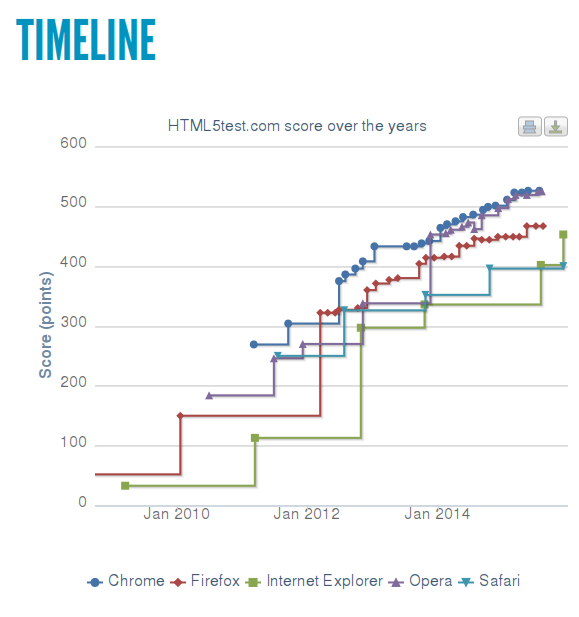
\includegraphics[width=0.8\textwidth,natwidth=610,natheight=642]{htmlSupport.png}
	\caption{Suporte das especificações do HTML nos navegadores}
    \label{fig:htmlSupport}
\end{figure}

%}}}
\section{ANDROID}
%{{{

É um sistema operacional open-source desenvolvido pela Google. Utiliza
o kernel Linux . Softwares para Android são geralmente escritos em Java
e executados através da máquina virtual Dalvik.

É similar a máquina virtual Java, mas roda um formato de arquivos
diferenciado (dex), otimizados para consumir pouca memória, que
são agrupados em um único Android Package (apk) Android permite a
renderização de documentos HTML através de sua própria API WEBVIEW.
Ou através do navegador disponibilizado por padrão, ou outros de
terceiros como o Google Chrome, Firefox, Opera, etc.

No quesito jogos para dispositivos móveis é preferível disponibilizar
os jogos através da interface nativa pois dá a sensação de
continuidade para com os demais aplicativos instalados no dispositivo.

%}}}
\section{DETECÇÃO DE RECURSOS}
%{{{
Visto que nenhum navegador implementa as especificações HTML
completamente cabe ao desenvolvedor detectar os navegadores que não
comportam as necessidades tecnológicas dos aplicativos que cria. Ao
deparar-se com uma funcionalidade faltante o desenvolvedor tem duas
possibilidades: notificar o usuário sobre o problema ou utilizar
polyfills.

Polyfills são recursos que simulam uma funcionalidade não
disponível nativamente nos navegadores. A biblioteca Gears
https://developers.google.com/gears é um exemplo. Gears
serve para prover recursos de Geolocalização para navegadores que
não implementam a especificação do HTML5. 

Essa capacidade de suportar tecnologias que não estão ainda
disponíveis (ou nunca estarão no caso de dispositivos legados)
através de polyfills é uma das características que faz a WEB uma
plataforma de tão grande abrangência. Novas tecnologias são criadas a
todo o momento; entretanto, o suporte a essas funcionalidades geralmente
não acompanham o passo das inovações. E ainda assim os usuários
podem se beneficiar de uma taxa substancial delas através de polyfills.

Algumas funcionalidades do HTML, como geolocalização e vídeo
foram primeiramente disponibilizadas através de plugins. Outras
funcionalidades, como o Canvas, podem ser totalmente emuladas via
JavaScript \autocite{diveIntohtml}.

Detectar suporte aos variados recursos do HTML5 no navegador
pode ser uma tarefa entediante. É possível implementar testes para
cada funcionalidade utilizada abordando os detalhes de implementação
de cada uma ou então fazer uso de alguma biblioteca especializada
neste processo. O Modernizr é uma opção open-source deste tipo de
biblioteca, este gera uma lista de booleanos sobre grande variedade dos
recursos HTML5, dentre estes, geolocalização, canvas, áudio, vídeo e
armazenamento local.

A quantidade de especificações que um aplicativo complexo como um jogo
utiliza pode ser bem grande, e muitas vezes é difícil dizer qual quais
navegadores implementam o quê. Uma boa referência do suporte a recursos
nos navegadores é o site http://caniuse.com/.

%}}}
\section{RENDERIZAÇÃO}
%{{{

Renderização é parte fundamental de muitos jogos. As tecnologias atualmente existes são o SVG e Canvas.

\subsection{SVG}
%{{{
SVG (\textit{Gráficos de vetores escaláveis}), é uma linguagem
baseada em XML especializada na criação de vetores bidimensionais
\autocite{html5mostwanted}. Por usar XML SVG permite a utilização da
API do DOM para manipular os elementos.

Entre os benefícios do SVG encontram-se:
\begin{itemize}
\item Não há diferença de qualidade em resoluções pois os vetores são escaláveis;
\item Suporta animações nativamente;
\item Conta com integração através da api do DOM. Tornando simples a integração com as outras tecnologias da web.
\end{itemize}

Um aspecto negativo do SVG é que é muito difícil atingir a
perfeição na posição dos pixels, por ser uma linguagem vetorizada
\autocite{html5mostwanted}.

\begin{figure}
\centering
\begin{verbatim}

<svg height="100" width="100">
  <circle cx="50" cy="50" r="40" stroke="black" stroke-width="3"/>
  Sorry, your browser does not support inline SVG.
</svg>

\end{verbatim}
\caption{Círculo em SVG.}
\end{figure}
%}}}
\subsection{CANVAS}
%%{{{

A tag \textit{canvas} define uma camada de mapa de bits em documentos
HTML que pode ser usada para criar diagramas, gráficos e animações
2D. Foi criada pela Apple em 2004 para renderizar elementos de interface
no Webkit, logo foi adotado por outros navegadores e se tornou um
padrão.

A API canvas cresceu com o tempo, e algumas funcionalidades - como
suporte a texto, foram adicionadas tardiamente. E alguns navegadores
lançaram antes da especificação estar completa e hoje tem problema
de suporte para essas áreas \autocite{diveIntohtml}. Apesar de muitas
vezes incompleto, o canvas é suportado em todos os maiores navegadores
à partir do Internet Explorer 9. Não obstante existe a possibilidade de utilizar
a biblioteca https://github.com/google/canvas-5-polyfill para
suprir aos navegadores que ainda não implementaram, os últimos recursos
da especificação CANVAS, como o recurso de desenhar elipses e o caminho 2D.

Apesar de ser geralmente bem suportado nos navegadores atuais, canvas
ainda sofre de problemas de performance. Para navegadores antigos -
abaixo do Internet Explorer 9 - existe o polyfill Explorer Canvas
do Google, que emula em JavaScript as funcionalidades do canvas. O
FastCanvas é uma iniciativa híbrida para Android que busca mitigar os
problemas de performance do Canvas com uma API nativa. Não obstante, o
FastCanvas não suporta a especificação do canvas completamente, não
permite ser integrado com outros elementos do DOM.

Em um documento HTML, Canvas é um retângulo onde pode-se usar
JavaScript para desenhar \autocite[pp. 113]{diveIntohtml}.

Canvas tem uma característica peculiar quanto ao seu tamanho.
Em suma existem dois tamanhos, o tamanho do elemento e da superfície de
desenho. Quando o tamanho do elemento é maior do que o da superfície
de desenho do documento escala a superfície de desenho para preencher o
elemento, o que pode gerar resultados inesperados.

Algumas outras fraquezas do canvas são:
\begin{itemize}
\item{Não há suporte a animações}
\item{Não é possível alterar uma parte já desenhada a não ser sobrescrevendo ou pintando o canvas novamente}
\item{Por ser um vetor de pixeis não existe possibilidade de utilização do DOM nem seus eventos, limitado muito a iteratividade}
\end{itemize}

O canvas até aqui descrito trata-se de sua forma, ou contexto 2D. A
especificação 3D do canvas é o WebGl.

%}}}
\subsection{WEBGL}
%{{

WebGL é uma API JavaScript para desenhar gráficos em três dimensões.
Apesar de ter sido desenvolvido com foco em 3D, WebGL pode ser
utilizados para 2D também \autocite[pp. 6]{3daps}. Os primeiros
rascunhos do WebGL iniciaram em 2006, não obstante o grupo de trabalho
não foi formado até 2009. E a primeira versão do foi lançada em
2011.

A especificação do WebGL foi desenvolvida baseando-se em OpenGL,
especificamente OpenGL ES 2.0, uma versão do OpenGL otimizada para
dispositivos móveis. O órgão que especifica o WebGL é o mesmo que
especifica o OpenGL: Kronos Working Group.

O elemento do DOM que provê a interface do WebGL é o canvas, no contexto 3D.
Essa integração com o DOM permite que o WebGL seja manipulado assim como os demais elementos HTML.

É digno de nota que é recomendável se testar WebGL em todos os navegadores
e plataformas alvo. Pode haver diferenças substanciais de performance em
plataformas diferentes e em navegadores diferentes. Existe também uma lista
de placas gráficas com drivers bloqueados por não funcionarem corretamente no
Firefox \autocite[pp.42]{3daps}.

WebGL só se tornou uma possibilidade performática para jogos
pois parte do seu processamento pode ser delegado para a GPU. A
especificação é composta por uma API de controle em JavaScript e o
processamento shaders. Shaders são responsáveis por grande parcela dos
efeitos 3D e são executados do lado da GPU.

\subsection{Shaders}

Shaders definem níveis de cor ou efeitos especiais sobre um modelo 2d
ou 3D. Contam com grande performance, possibilitando conteúdo em tempo
real - como no caso dos jogos - por executarem dentro da GPU.
São utilizados no cinema, em imagens geradas por computadores e vídeo games.

Existem dois shaders principais, de vértices e fragmentos.
Shaders de vértices são chamados para cada vértice sendo desenhado
definindo suas posições e shaders de fragmentos a cor para cada pixel
a ser desenhado \autocite[pp.15]{3daps}.

\subsection{Bibliotecas OpenGL}

CocoonJS é uma aplicativo híbrido que preenche a fraca implementação
de WebGL nos dispositivos móveis possibilitando se desenvolver em
WEBGL, CSS. Conta com suporte a dispositivos legados à partir do
Android 2.3 e IPhone 5.

Treejs é uma abstração sobre WebGL que permite os autores se focarem
na criação de conteúdo para web, ao invés de dispenderem tempo manipulando
os detalhes da WebGL. Possibilita trabalhar com efeitos, luzes, cenas
e outras abstrações em detrimento de shaders, vértices, e conceitos mais
primitivos.

\subsection{Otimizações}
CPU? JavaScript, DOM, etc.
GPU?

- Texture compression
- Mipmaps (LOD)
- Draw calls

Um site interessante para explorar exemplos WebGL avançados é o blog
http://learningwebgl.com que conta com tutoriais cobrindo áreas como
diferentes tipos de iluminação, carrecamento de modelos em json,
gerenciando eventos do mouse e teclado; e como renderizar uma cena WebGL
em uma textura \autocite[pp.42]{3daps}.

Apesar da relevância, WebGL não foi utilizada no trabalho pois ainda
não está completamente especificada e a dificuldade e escopo do
projeto aumentariam muito se tivessem de incluir um jogos 3D.

Uma tecnologia que se integra profundamente como ambientes virtuais
em três dimensões criados via OpenGL é o WebVR.
%}}}
\subsection{WEBVR}
%{{{
Segundo \cite{virtualReality} realidade virtual é uma experiência em
que o usuário é efetivamente imerso em um mundo virtual responsivo.
Realidade virtual é uma área nem tão nova mas que recebeu interesse
renovado recentemente. Isso se dá, pelo menos me parte, pela
massificação dos dispositivos móveis inteligentes. O hardware
necessário para fornecer uma experiência minimamente viável como
acelerômetros, câmeras e telas de alta resolução está disponível
em praticamente todos os dispositivos comercializados.

Realidade virtual é uma área de grande interessa para os produtores
de jogos, pois pode oferecer alto nível de imersão nos já
interativos e desafiadores ambientes dos jogos.

A WebVR é uma especificação que pretende trazer os benefícios
da realidade virtual para dentro do mundo da WEB. Em termos simples
a especificação define uma forma de traduzir movimentos de
acelerômetros e outros sensores de posição e movimentos para dentro
do contexto de uma um contexto 3D através de JavaScript.

Atualmente a especificação do WebVR se encontra em fase de rascunho e
as últimas versões do Firefox, e versões compiladas manualmente do
Google Chrome já permitem a utilização.


%}}}
\section{WebCL}
%{{{
É uma API em JavaScript para o recursos de OpenCL que permitem
computação paralela com grandes ganhos de performance. Aplicativos
como moteres de física e renderizadores de imagens, ambos relevantes
para os jogos, podem se beneficiar grandemente de processamento feito em
paralelo, possivelmente na GPU. OpenCL é um framework para escrever
programas que funcionem em plataformas com diversas unidades de
processamento, assim como WebGL e WebCL é especificada e desenvolvida
pelo grupo Kronos.

A primeira versão da especificação foi no início de 2014 mas até
então nenhum navegador implementa o definido.
%}}}
\section{CODECS}
%{{{
Para falar sobre audio e vídeo precisamos primeiramente introduzir o
conceito de codecs. Codec - é o algorítmo usado para encodificar o
video em um conjunto de bits \cite{diveIntohtml}.

Codecs é uma área problemática do HTML5. Segundo \cite{diveIntohtml}
não existe uma única combinação de containers e codecs que funcionem
em todos os navegadores.

\section{AUDIO}
%{{{
Áudio é um componente vital para oferecer imersão e feddback
aos usuários de jogos. Efeitos de som e música podem servir como
mecanismo. Por outro lado, jogadores tem baixa tolerância a volume,
deve ser utilizado com cautela.

Segundo \cite{browserGamesTechnologyAndFuture} em sido difícil
construir aplicações sofisticadas e interativas sem a utilização de
plugins para áudio.

O componente de áudio é especialmente útil para jogos de ação
\autocite{browserGamesTechnologyAndFuture}.

\subsection{TAG AUDIO}

A tag <audio> define um som dentro de um documento HTML. Quando o
elemento é renderizado pelos navegadores, ele carrega o conteúdo que
pode ser reproduzido pelo player de audio do navegador. Existem muitas
discrepâncias entre os formados aceitáveis pelos navegadores. É um
tanto limitada quanto comparada ao áudio de múltiplos canais
disponibilizados por SDKs nativas.

\subsection{API DE AUDIO}

É uma interface de audio experimental para JavaScript. Provê maior
flexibilidade na manipulação de audio. Essa tecnologia é muito mais
nova do que a tag áudio.
Abaixo segue alguns dos codecs de audio tradicionais:

\begin{itemize}
    \item{MP3: comum, mas não é livre de patentes}
    \item{ACC: advanced audio coding, is patent encumbered} \item{Vorbis - patent free}
\end{itemize}

A figura \ref{fig:audioCodecs} é um comparativo interessante sobre os
formatos existentes, considerando o fator taxa de bits versus qualidade.

\begin{figure}
    \centering
    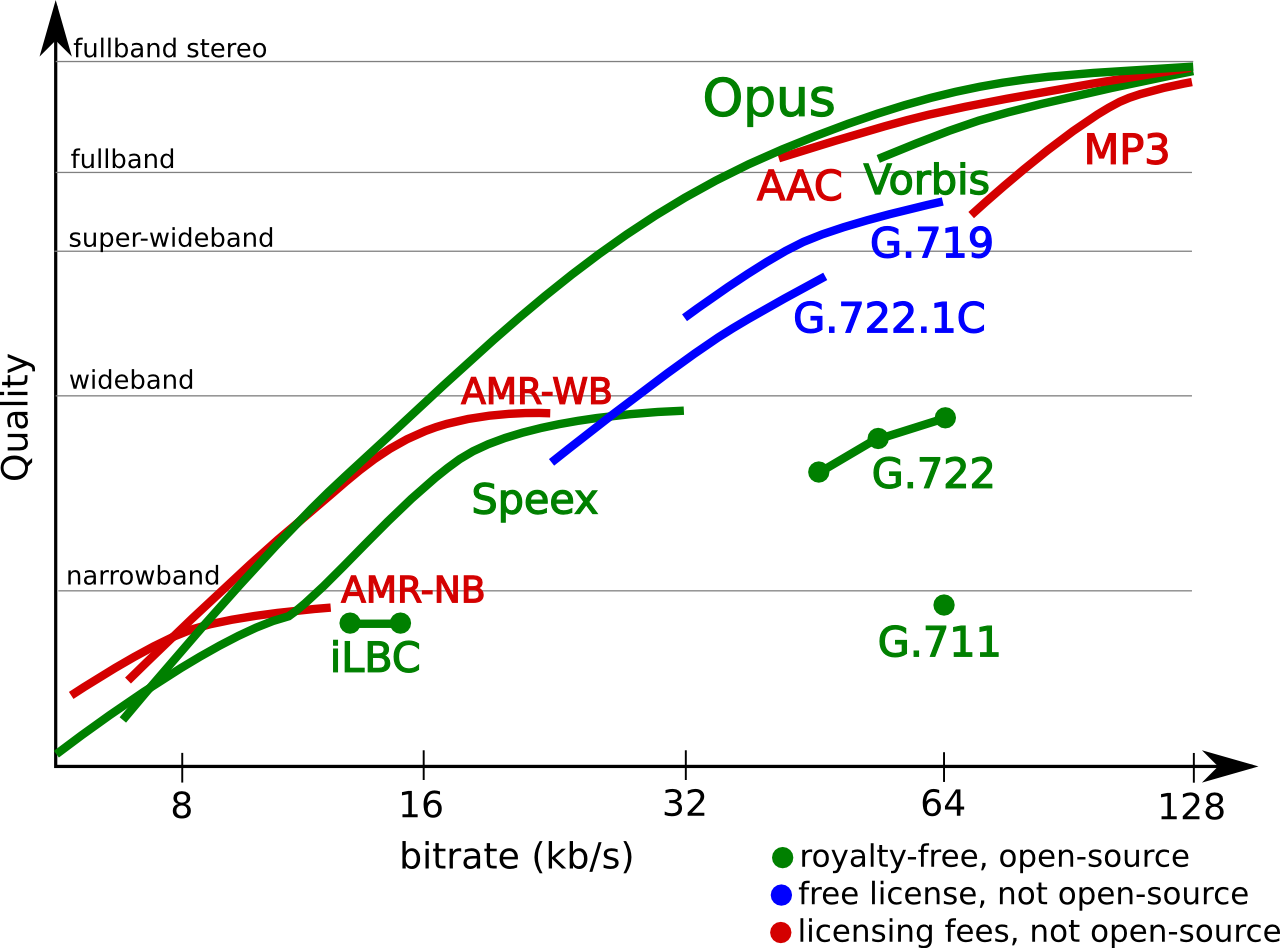
\includegraphics[width=0.8\textwidth,natwidth=610,natheight=642]{codec.png}
	\caption{Comparação de codecs de áudio}
    \label{fig:audioCodecs}
\end{figure}

%}}}

\section{VIDEO}
%{{{
Antes do HTML5 era impossível adicionar vídeos nas páginas sem a utilização de algum plugin.

A especificação define uma tag \textit{video} que pode ser embida em uma página HTML. Segundo \cite{diveIntohtml} não existem restrições quando ao codec de vídeo ou áudio, um elemento vídeo pode fazer referência a múltiplos arquivos de vídeos, cabe ao navegador decidir qual arquivo de fato será executado.

Os navegadores não concordam em qual formato de vídeo suportar.
Uma tag vídeo pode apontar para vários arquivos em diversos formatos, e os navegadores que suportarem determinado irão escolhê-lo.

Um formato de vídeo é a combinação de várias tecnologias.

AVI e MP4 são apenas containers de formatos. Como um arquivo zip, podendo conter qualquer coisa dentro de si \autocite{diveIntohtml}.

Existem formatos desenvolvidos especificamente para a Web. Buscam uma razão de tamanho e qualidade aceitável, mas prezando por tamanho. A maioria dos codecs de vídeo não mudam todo o conteúdo de um quadro para o próximo, possibilitando maiores taxas de compressão, que resulta em arquivos menores \autocite{diveIntohtml}.

O projeto \textit{Vídeo for Everybody} \begin{verbatim} http://camendesign.com/code/video_for_everybody \end{verbatim} é um polyfill que recorre à flash quando o vídeo não é suportado pelo navegador.


Segue uma lista de alguns dos containers de video:
\begin{itemize}
    \item{MPEG4}
    \item{Flash Video}
    \item{Ogg} (for video Theora), (audio Vorbis)
    \item{WebM}
    \item{Matroska}
    \item{Audio Video Interleave}
\end{itemize}

Alguns codecs de vídeo
\begin{itemize}
    \item{H.264, is one of the video codecs mandated by the Blue-Ray specification}
    \item{Theora, native in Linux}
    \item{VP8 royality free from Google}
\end{itemize}

%}}}
%}}}
\section{ARMAZENAMENTO}
%{{{
Uma das grades limitações do HTML era a ausência de capacidade de
armazenamento de dados no lado do cliente. Antes do HTML5 a única
alternativa era usar cookies, os quais tem um armazenamento de no
máximo 4k e trafegam em toda a requisição, tornando o processo lento.
Essa área era ode as aplicações nativas detinham grande vantagem
sobre as aplicações web. O HTML5 solucionou este problema introduzindo
várias formas de armazenamento de dados \autocite{html5Tradeoffs}.

Armazenamento local é um recurso importante para jogos, tanto por
diminuir a latência da persistência na rede, quanto para possibilitar
um experiência offline.

Existem algumas especificações sobre armazenamento, mas a grande
parte delas não conta como suporte completo em todos os navegadores
comuns, um polyfill interessante para Web Storage  e IndexedDB é o
projeto localForge \textit{https://github.com/mozilla/localForage} da
Mozilla.

\subsection{WEB SQL}

A especificação Web SQL introduz uma API para manipular banco de dados
relacionais em SQL. A especificação suporta transações, operações
assíncronas e um tamanho de armazenamento substancial: 5 megabytes, o
qual pode ser estendido pelo usuário.

O grupo de trabalho do Web SQL iniciou-se em 2010 e foi suspendido ainda
como rascunho. Apesar de ser um recurso desejável para muitos
desenvolvedores, foi descontinuada pelos motivos descritos abaixo.

Segundo \cite{diveIntohtml}
\begin{quote}
Todos os implementadores interessados em Web SQL utilizaram a mesma
tecnologia (Sqlite), mas para a padronização ficar completa é
necessário múltiplas implementações. Até outro implementador se
interessar em desenvolver a especificação a descrição do dialeto SQL
apenas referencia o SQLITE, o que não é aceitável para um padrão.
\end{quote}

Não obstante, a especificação ainda é suportada pelo Google
Chrome, Safari, Opera e Android, entre outros. Mas até que outros
implementadores se prontifiquem a especificação continuará suspensa.
No lugar do Web SQL a W3C recomenda a utilização do Web Storage e do
IndexedDB.

\subsection{WEB STORAGE}

Web Storage, também conhecido como Local Storage, provê uma forma de
armazenar os dados como chave valor dentro do navegador. Os dados são
persistidos mesmo que o navegador seja fechado.

É um recurso similar a cookies, contudo algumas diferenças
substanciais são perceptíveis. Web Storage não requer que os dados
sejam trafegados como cabeçalhos nas requisições. Também provê
maiores espaços de armazenamento quando comparado a cookies.

A tecnologia começou como parte da especificação do HTML5 mas agora
conta com um documento próprio mantido pela W3C. A especificação é
suportada pela grande maioria dos navegadores populares.

A especificação oferece duas áreas de armazenamento, o armazenamento
local e de sessão. O armazenamento local é persistido por domínio
e outros scripts provindos deste mesmo domínio poderão fazer uso da
informação. O armazenamento de sessão é para informações que podem
variar de aba para aba e que não é interessante que sejam persistidos
para demais acessos além do atual.

A API do Web Storage é simples, consistindo em uma interface para
buscar dados e outra para armazenar, no formato chave/valor.

\begin{figure}
\centering
\begin{verbatim}
// Store value on browser for duration of the session
sessionStorage.setItem('key', 'value');

// Retrieve value (gets deleted when browser is closed and re-opened)
alert(sessionStorage.getItem('key'));

// Store value on the browser beyond the duration of the session
localStorage.setItem('key', 'value');

// Retrieve value (persists even after closing and re-opening the browser)
alert(localStorage.getItem('key'));

\end{verbatim}
\caption{Web Storage na prática}
\label{fig:WebStorage}
\source{https://en.wikipedia.org/wiki/Web\_storage\#usage}
\end{figure}

A figura \ref{fig:WebStorage} exemplifica a utilização do Web Storage,
para utilizar o armazenamento de sessão utiliza-se o objeto sessionStorage. Já
para utilizar o armazenamento local utiliza-se o objeto localStorage.

Web Storage é uma solução simples que comporta muitos casos de uso.
Não obstante muitas vezes é necessário um controle mais refinado
sobre os dados, ou mais performance em uma base de dados massiva. Para
responder a estes desafios existe a especificação do IndexedDB.

\subsection{IndexedDB}
%{{{
IndexedDB é um banco de dados que suporta o armazenamento de grandes
quantidades de dados no formato de chave/valor o qual  permite alta
performance em buscas baseadas em índices. A tecnologia é uma recomendação
da W3C desde janeiro de 2015 e suportada, pelo menos parcialmente, por
praticamente todos os navegadores populares.

Inicialmente IndexedDB permitia operações síncronas e assíncronas.
Não obstante, a versão síncrona foi removida devido a falta de
interesse da comunidade. Operações assíncronas permitem que
aplicativos JavaScript nunca esperam pelo resultado para continuar a
execução. Outrossim, cada interação com o banco de dados é uma
transação que pode retornar um resultado ou um erro. Os eventos da
transação são internamente eventos DOM cuja propriedade \textit{type}
do elemento foi setada para \textit{success} ou \textit{error}.

Ao invés de tabelas, IndexedDB trabalha com repositórios de objetos.
Cada entrada, tupla em SQL, de um determinado repositório pode ser de
um formato diferenciado, com exceção da chave única que deve estar
presente em cada uma das entradas.

\begin{figure}
\centering
\begin{verbatim}
	var db;
	var request = window.indexedDB.open("Mydb", 9);
	request.onsuccess = function(event) {
		db = event.target.result;
		var transaction = db.transaction(["customers"], "readwrite");
		var objectStore = transaction.objectStore("customers");
		var request = objectStore.add({email: "mymail@domain.com", name: "foo"});
		request.onsuccess = function(event) {
			console.log('customer added')
		};
	}
\end{verbatim}
\caption{Adicionando um cliente em IndexedDB.}
\label{fig:IndexedDB}
\end{figure}

A figura \ref{fig:IndexedDB} demonstra um exemplo simplificado da
utilização do IndexedDB, como cada iteração com o banco de dados é
construído através de uma nova requisição e o tratamento do resultado
é dado dentro de eventos.

Apesar de ser desenvolvido com objetivo de ser uma solução para todas
as necessidades de armazenamento no Frontend IndexedDB ainda sofre
algumas limitações.

Abaixo segue uma lista com algumas das limitações do IndexedDB.

\begin{itemize}
\item Tem limites de armazenamento e as regras variam de navegador para navegador.
\item O comportamento em abas anônimas não está especificado e os resultados também variam.
\item Existe uma pequena probabilidade de os dados se perderem, no caso do Firefox a API não espera confirmação do sistema operacional para considerar um dado válido, essa foi uma escolha em detrimento de performance.
\item Não existe a possibilidade de fazer buscas em textos como o \textit{LIKE} do SQL.
\item o usuário pode configurar o navegador para não aceitar armazenamento local para determinado domínio.
\end{itemize}

%}}}

A característica assíncrona do IndexedDB, é fundamentada na
premissa de não perturbar o fluxo principal da aplicação enquanto
processamento não vital, e possivelmente demorado, ocorre. Outra
tecnologia da web que utiliza os mesmos princípios é o Web Workers.

%}}}
\section{WEB WORKERS}
%{{{

É uma API que possibilita executar vários scripts
(\textit{threads}) JavaScript ao mesmo tempo. O script que cria uma
thread é chamado de pai da thread, e a comunicação entre pai e filhos
pode acontecer de ambos os lados através de mensagem encapsuladas
em eventos. Um script que não seja pai de uma thread não pode se
comunicar com ela, a não ser que a thread seja em modo compartilhado.

O contexto global (objeto \textit{window}) não existe em uma
thread, no seu lugar o objeto \textit{DedicatedWorkerGlobalScope}
pode ser utilizado. Workers compartilhados podem utilizar o
\textit{SharedWorkerGlobalScope}. Estes objetos contém grande parte das
funcionalidades proporcionadas pelo window com algumas exceções, por
exemplo threads não podem fazer alterações no DOM.

%}}}
\section{OFFLINE}
%{{{

Não é extraordinário que um jogo tenha que ser reverso para um estado
válido anterior por motivo de um erro na base de dados \autocite[pp.
5]{browserGamesTechnologyAndFuture}.

\subsection{Aplicações offline}
Na sua versão mais simples, um aplicativo offline é um conjunto de
URLs para arquivos HTML, CSS, JavaScript, imagens ou qualquer outro tipo
de recurso \autocite{diveIntohtml}.

%}}}
\section{ENTRADA DE COMANDOS}
%{{{
Na construção da grande maioria dos jogos é muitas vezes
imprescindível grande flexibilidade na gestão de entrada comandos.
Esta necessidade amplia na criação de jogos multiplataforma, em
determinadas plataformas a entrada de comandos pode-se dar través de
teclado, em dispositivos móveis através tela sensível ou sensor de
movimentos.

O HTML5 trata todos estes casos abstratamente na forma de eventos, os
quais podem ser escutados através de \textit{listeners}. Os eventos
básicos são: keydown (tecla baixa), keyup (tecla solta) e keypress
(tecla pressionada).

\subsection{Acelerômetro}

%}}}
\section{HTTP/2}
%{{{

HTTP/2 é a última verão do protocolo de trocas de documentos da WEB. Quando um cliente requisita algum 
documento de um servidor esta requisição é feita, geralmente, através do protocolo HTTP2.

A versão 2 trouxe grandes benefícios em potencial para performance, visto que o htt2 abre apenas
uma conexão por host. 
Htt2 também não recomenda a utilização de minificação nos arquivos, o que antes era um benefício 
de performance agora pode ser um malefício. No contexto dos jogos onde o carregamento da tela inical 
pode demorar muito isso é um fator vital.

%}}}
\section{DEBUG}
%{{{

\subsection{Source Maps}

Source Maps é uma tecnologia que permite mapear códigos fontes
minificados para seus respectivos originais. Este recurso é
interessante pois permite que os desenvolvedores visualizem o código
fonte em sua versão original, legível, enquanto entregam ao usuário
final a versão minificada, optimizada para performance.
Para o usuário final não há diferença pois Source Maps são
carregados apenas se as ferramentas de desenvolvimento estão abertas e
com a funcionalidade de Source Maps habilitada.

Source Maps foi desenvolvido como um trabalho em conjunto entre a
Mozilla e Google em 2010, atualmente na terceira revisão o projeto é
considerável estával e não recebe modificações na especificação
desde 2013.

As ferramentas de desenvolvimento do Google Chrome e Firefox permitem a
utilização de Source Maps.

É possível informar o navegador a localização do arquivo original
seguindo a seguinte sintaxe.

\begin{verbatim}
//# sourceMappingURL=/path/to/script.JavaScript.map
\end{verbatim}

Ou através de cabeçalhos HTTP como demostrado abaixo.

\begin{verbatim}
X-SourceMap: /path/to/script.JavaScript.map
\end{verbatim}

Arquivos de Source Map contém metadados sobre os arquivos fonte e
algumas outras configurações.
Para gerar os arquivos é possível utilizar ferramentas como o
https://github.com/mishoo/UglifyJS2.

\subsection{Debug 3D}
Debugar aplicativos 3D pode ser complexo, o debugger do chrome é uma boa opção.

%}}}
\section{DISPONIBILIZAÇÃO DA APLICAÇÃO}
%{{{
Aplicativos baseados na web não requerem instalação ou atualizações
manuais e sua distribuição é superior ao estilo convencional de
aplicações desktop \autocite{browserGamesTechnologyAndFuture}.

Links com manifestos

\subsection{INSTALAÇÃO}
%{{{
Este método é benéfico pois possibilita ao usuário a mesma
experiência ao adquirir uma aplicação normal. Este tipo de
aplicação é comummente referido como "híbrido".
%}}}

%}}}
\section{TRABALHOS SIMILARES}
%{{{
\cite{crossPlatformMobileGame} elaborou uma revisão de aspectos do
HTML5 através da construção de um jogo. O autor foca muito nos
aspectos de criação de jogos e feedback do desenvolvimento. Troca
de tecnologias e não especificamente nas limitações conforme o meu
trabalho. Em outras palavras seu escopo é mais genérico e não tão
preciso quanto este
%}}}
